% !TeX root = ../main.tex
\section{Reading the Training Signal: Full Construction and Results}
\label{app:mechanism}

This appendix expands \S\ref{sec:mechanism}. It measures what each method's update pushes
toward, from the training data itself rather than from outcomes.

\subsection{Putting two losses on one probe}

Both methods weight the candidates of a group and step along the weighted sum. For a group
of candidates $\{y_g\}$ each is assigned a weight $w_g$:

\begin{itemize}\itemsep2pt
  \item \textbf{PTO / DPO:} $w_g = +1$ on the logged \emph{chosen}, $-1$ on
  \emph{rejected}, $0$ otherwise --- i.e.\ the literal $\tau$-filtered pair.
  \item \textbf{GRPO:} $w_g = (r_g - \mathrm{mean}_g\,r)/\mathrm{std}_g\,r$, the
  standardized advantage that scales each completion's gradient.
\end{itemize}

\noindent
Weights are then rescaled \emph{within each group} to $\sum_g |w_g| = 2$, which is DPO's
natural scale. This rescaling is what makes the two comparable: without it, GRPO's weights
carry the group's reward spread and every cross-method quantity becomes a scale artifact.
Groups lacking either sign are dropped --- for PTO that means a branch point the $\tau$
filter left unpaired, which never trained.

Two readouts are taken off the weighted groups:

\begin{itemize}\itemsep2pt
  \item \textbf{Lexical push} $\sum_g w_g\,\phi(y_g)$, averaged over groups with a standard
  error, for a feature $\phi \in \{$length, question marks, affirmation cues, over-praise
  cues$\}$. Units are chosen-minus-rejected, so $0$ means the update is indifferent to the
  feature. This is exact, uses no embeddings, and covers every group. The affirmation and
  over-praise cue sets are deliberately the \emph{same} regexes used for the
  conversation-side checks in \S\ref{sec:hacking}, so the two sides are able to agree.
  \item \textbf{Update direction} $\mathrm{normalize}(\sum_g w_g\, e(y_g))$ in sentence-
  embedding space --- a mass-mean probe generalized to an arbitrary weighting.
\end{itemize}

\paragraph{A probe audit, and what it disqualifies.}
Directions are only usable where they are actually estimated. Scoring each half of an
iteration's groups with the other half's direction gives a split-half reliability of
$0.15$--$0.32$ for a \emph{per-iteration} PTO direction --- two halves of one iteration point
almost independently --- so per-iteration direction results are estimation noise and we do
not report them. Pooled over iterations the directions are usable ($0.60$ PTO, $0.91$ GRPO),
and all direction results below are pooled. Cross-arm cosines are additionally divided by the
attenuation ceiling $\sqrt{r_a r_b}$, since two noisy estimates cannot agree perfectly even
if identical. (For the same-groups rows of Table~\ref{tab:decomp} the correction
over-corrects, because both directions share their estimation noise; a corrected value above
$1.0$ is the tell, so those rows are read raw.)

\subsection{The affirmation push, per iteration}

\begin{figure}[h]
  \centering
  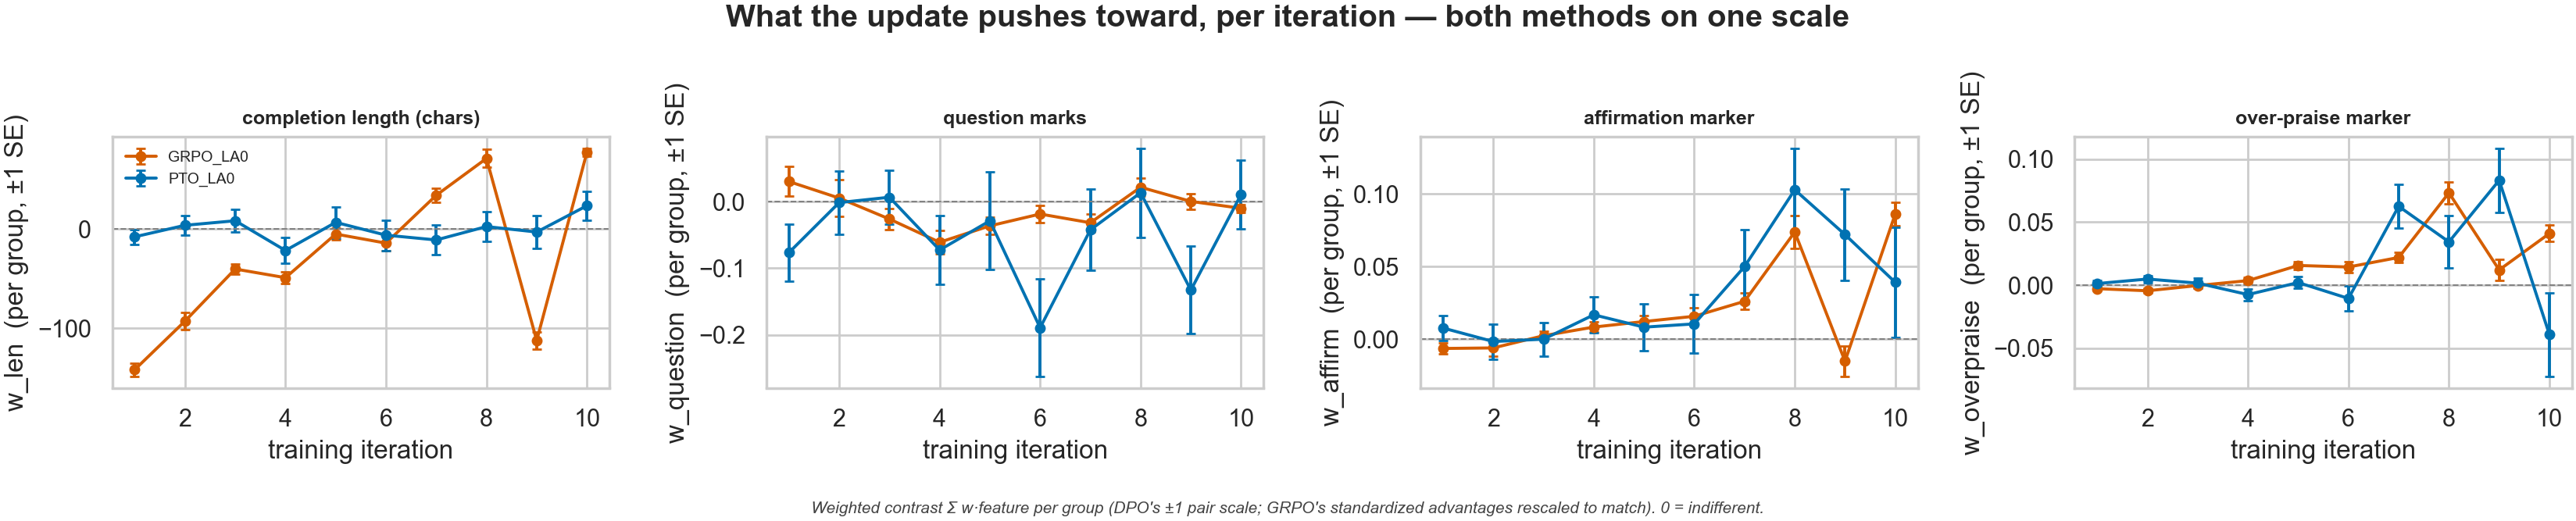
\includegraphics[width=\linewidth]{figures/update_lexical_push_gpt-4o-mini.png}
  \caption{Weighted affirmation contrast per training iteration, $\pm$ SE. Both arms rise;
  GRPO reaches $+0.086\,(\pm0.008)$ at iteration~10 and PTO peaks at $0.103\,(\pm0.029)$ at
  iteration~8 (its iteration-10 estimate, $0.039 \pm 0.038$, rests on far fewer groups --- see
  Table~\ref{tab:yield}). GRPO's series dips \emph{negative} at iteration~9, the same
  iteration at which the outcome grid dips (\S\ref{sec:results}), from a completely
  independent source.}
  \label{fig:push}
\end{figure}

\subsection{Generation versus selection}

\begin{figure}[h]
  \centering
  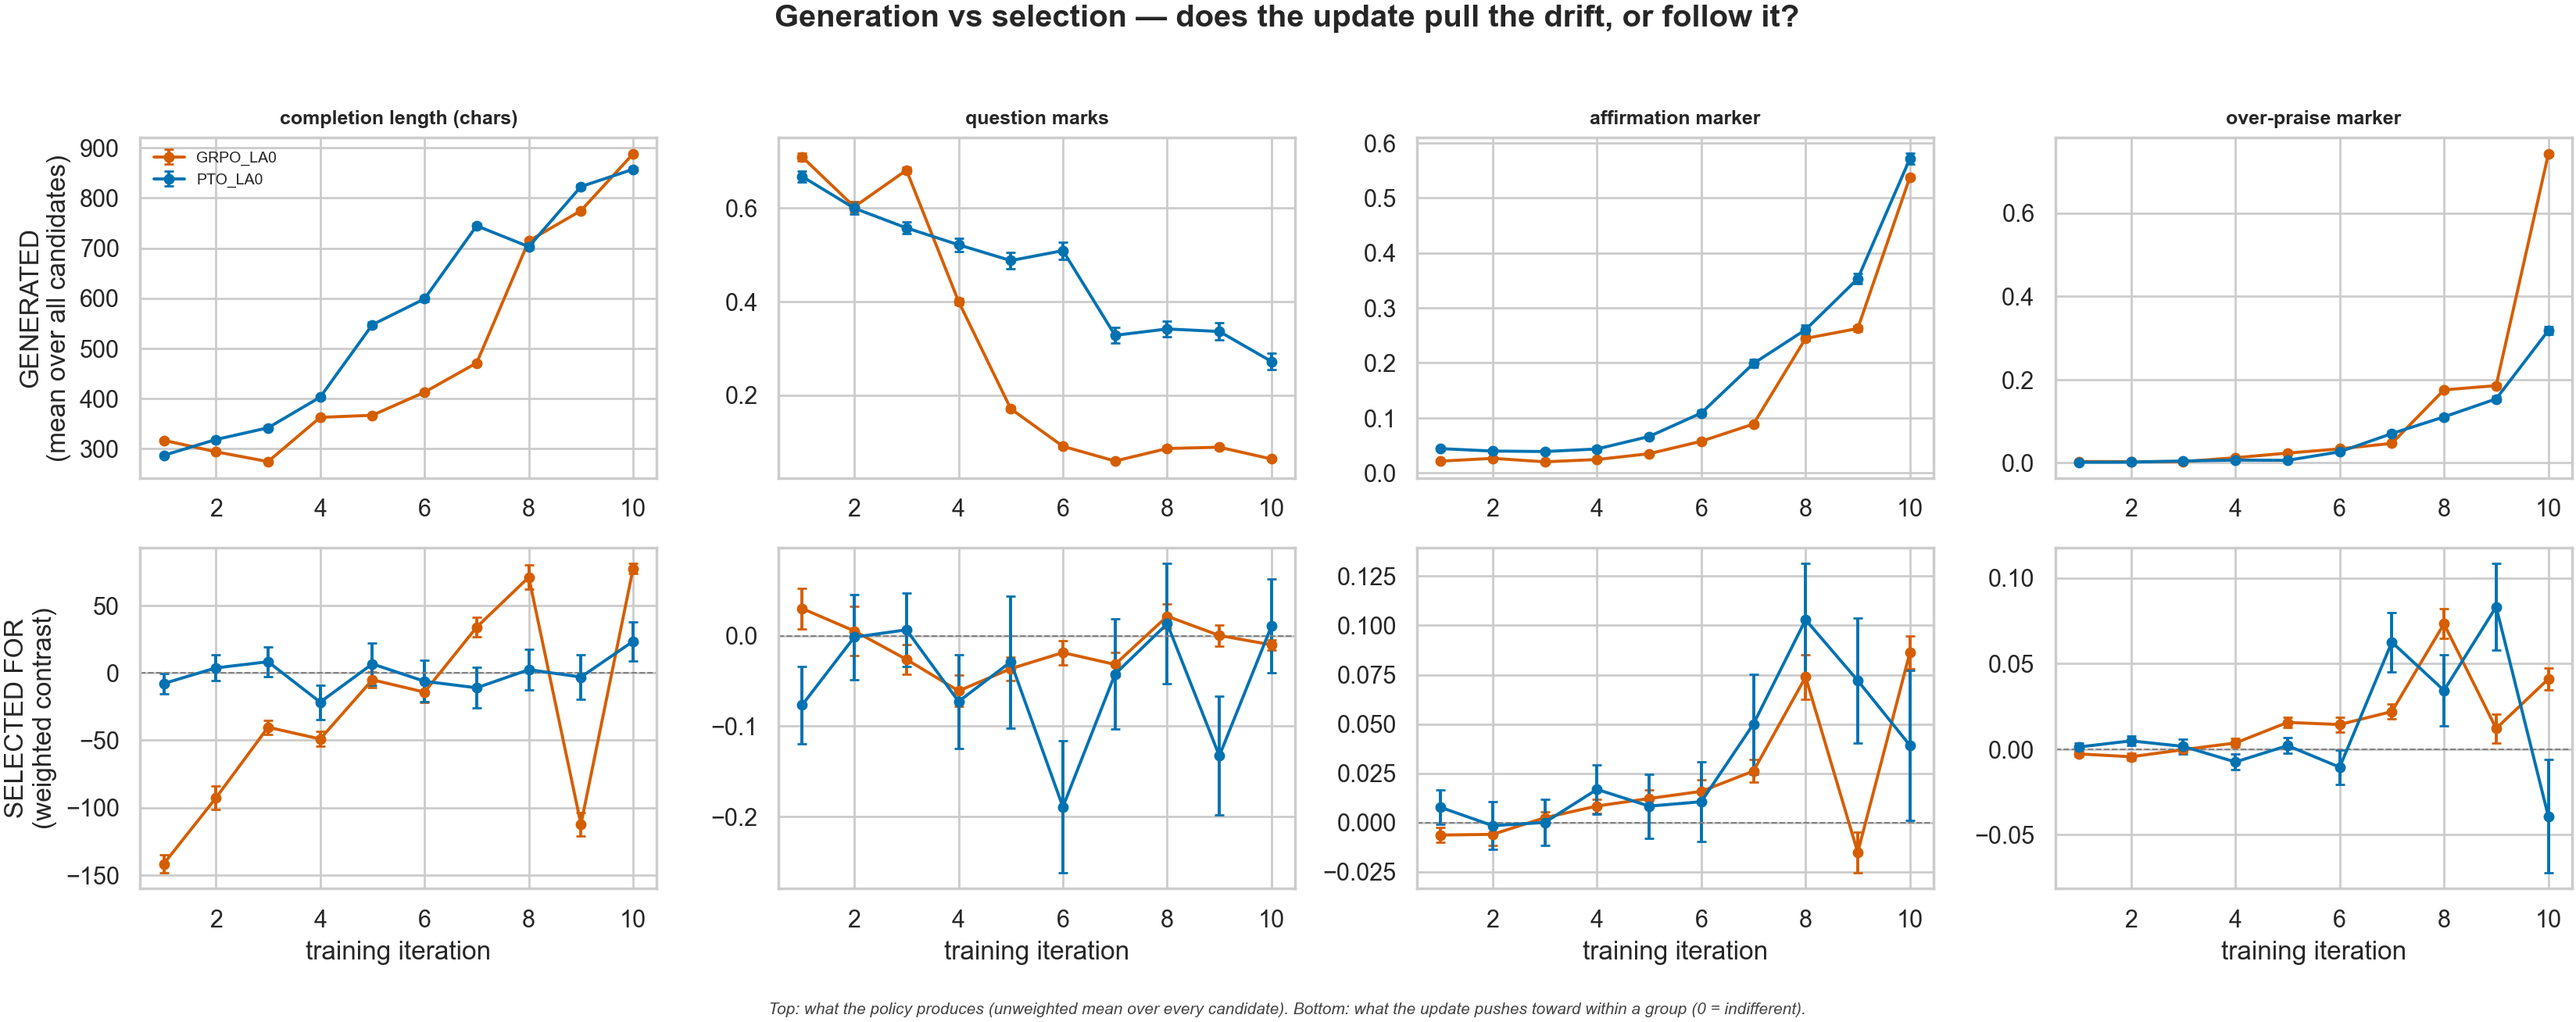
\includegraphics[width=\linewidth]{figures/generation_vs_selection_gpt-4o-mini.png}
  \caption{What the update \emph{selects for} (per-group weighted contrast) against what the
  policy \emph{generates} (unweighted mean over all sampled candidates). The pool moves an
  order of magnitude more than the selection pressure that produces it.}
  \label{fig:genvssel}
\end{figure}

Over all sampled candidates, mean affirmation-cue rate goes $0.021 \to 0.538$ (GRPO) and
$0.044 \to 0.571$ (PTO); over-praise cues reach $0.741$ of GRPO's candidates (PTO $0.318$);
question marks per candidate fall $0.710 \to 0.063$ (GRPO) and $0.668 \to 0.272$ (PTO).
Against a per-iteration selection pressure of ${\approx}0.01$--$0.10$, this is a compounding
on-policy loop rather than one strong pull.

\emph{Indexing note.} Training iteration $n$ samples from the iteration-start policy, so a
pool row describes the policy the evaluation set calls \texttt{model\_iter\_}$(n{-}1)$ ---
deliberately off by one from the selection contrast on the same row.

\subsection{Loss versus data}

\begin{table}[h]
  \centering\small
  \setlength{\tabcolsep}{4pt}
  \begin{tabular}{@{}lccc@{}}
    \toprule
    Comparison & cos & ceil. & corr.\\
    \midrule
    As trained (rule + data differ) & 0.267 & 0.844 & \textbf{0.317}\\
    Same groups (PTO), rule swap    & \textbf{0.908} & --- & ---\\
    Same groups (GRPO), rule swap   & \textbf{0.988} & --- & ---\\
    Same rule (group-rel.), data differ & 0.356 & 0.896 & 0.397\\
    Same rule (best-worst), data differ & 0.266 & 0.823 & 0.324\\
    \bottomrule
  \end{tabular}
  \caption{Decomposing the cross-method update-direction gap by applying each weighting rule
  to the other method's candidate groups. The rule contributes almost nothing; the data
  contributes almost everything. Same-groups rows are read raw (see the audit above).}
  \label{tab:decomp}
\end{table}

\subsection{Training-signal yield}

\begin{table}[h]
  \centering\small
  \begin{tabular}{@{}lrrrr@{}}
    \toprule
    & \multicolumn{2}{c}{PTO} & \multicolumn{2}{c}{GRPO}\\
    \cmidrule(lr){2-3}\cmidrule(lr){4-5}
    Iter & built & trained & built & trained\\
    \midrule
    1  & 949 & 782 & 1728 & 1660\\
    5  & 600 & 483 & 1888 & 1789\\
    10 & 410 & 281 & 2528 & 2484\\
    \midrule
    yield & \multicolumn{2}{c}{$0.82 \to 0.69$} & \multicolumn{2}{c}{$0.94$--$0.98$}\\
    margin & \multicolumn{2}{c}{$0.274 \to 0.196$} & \multicolumn{2}{c}{$0.379 \to 0.339$}\\
    \bottomrule
  \end{tabular}
  \caption{PTO's $\tau$ filter and its shrinking branch count cost it two-thirds of its
  training signal over the run, while GRPO trains on nearly every group it builds. A
  flattening PTO curve may partly be a data-starvation curve. Full per-iteration values in
  the released tables.}
  \label{tab:yield}
\end{table}

\subsection{Does the training push predict the outcome move?}

With the iteration index partialled out of both sides --- mandatory, since both the push
features and the evaluation deltas trend with training by construction --- GRPO's
per-iteration change in \mici{} tracks its affirmation push at $\rho = 0.647$ ($p = .043$),
its length push at $0.706$ ($p = .023$) and its over-praise push at $0.617$ ($p = .057$).
PTO's does not ($-0.492$, n.s.). This is the same direction as the endpoint \mici{} gap
(\S\ref{sec:hacking}), reached from the training data instead of from the transcripts. With
$n \le 10$ iterations per arm and no multiplicity correction it is a mechanism consistent
with the curves, not a demonstrated cause.
